\documentclass[11pt,a4paper]{article}
\XeTeXlinebreaklocale "zh"
\XeTeXlinebreakskip = 0pt plus 1pt minus 0.1pt
\usepackage[top=1in,bottom=1in,left=1.25in,right=1.25in]{geometry}
\usepackage{float}
\usepackage{fontspec}
\newfontfamily\zhfont[BoldFont=STHeiti]{STFangsong}
\newfontfamily\zhpunctfont{STFangsong}
\setmainfont{Times New Roman}
\usepackage{indentfirst}
\usepackage{zhspacing}
\zhspacing

% 代码展示
\usepackage{color}
\definecolor{bg}{rgb}{0.152941, 0.156863, 0.133333}
\usepackage{minted}
\usemintedstyle{monokai}
\setmonofont{DejaVuSansMono}

\usepackage{fancyvrb}  % 调整 Verbatim 中字体

% 调整 quotation 字体
\let\quotationOLD\quotation
\def\quotation{\quotationOLD\footnotesize}

\usepackage{pdfpages}  % 附上 pdf 版综合结果

\begin{document}

\title{实验零\ \ Verilog 作业}
\author{无36$\quad$李思涵$\quad$2013011187}
\maketitle


\section{作业思路}

\subsection{多路选择器}
\subsubsection{2-1 多路选择器}
2-1 多路选择器中,开关由一根控制线 $s$ 控制。$s$ 选择两个输入 $a, b$ 中的一个作为输出。

在经卡诺图化简之后,可以得到如下逻辑表达式
\[
  y = \bar{s}\cdot a + s\cdot b
\]
故先用非门得到 $\bar{s}$,再使用两个与门和一个或门,就可以得到正确的 $y$ 了。

\paragraph{消除冒险}
从卡诺图中可以看到,此时的电路是存在静态 1 冒险的。具体则是当 $a = 1, b = 1$,$s$ 由 1 变为 0 时,假设各个门延时相同,输出会由 1 跳变成 0,然后又跳变回 1。

为了消除冒险,我们可以引入冗余项 $a\cdot b$,这样就可以消除静态 1 冒险。

\subsubsection{4-1 多路选择器}
4-1 多路选择器则可以用三个 2-1 多路选择器来实现,即 $s_0$ 在 $c_0, c_1$ 之间,以及 $c_2, c_3$ 之间进行选择,$s_1$ 则在上面两个结果之间选择。

\subsection{三八译码器}
从三八译码器的卡诺图中可以看到,输出的每一位均可以直接表示为 $A_2, A_1, A_0$ 以及他们的反中三项的与。故用 3 个非门,8 个三输入与门即可实现。

\subsection{移位寄存器}
要实现一位寄存器,首先要实现具有异步复位的 D 触发器。其可以用与非门实现,方法在作业要求中提到了。

移位寄存器则可以通过 D 触发器的级联实现,即上一级的输出端 Q 对应的接到下一级的输入端 D,而最上级的输入端 D 接到整个移位寄存器的移位输入。

同时,为了实现同步置数功能,应该在电路中加入四个受 $load$ 信号控制的 2-1 多路选择器,在 $load$ 高电平选择并行数据。

\section{电路代码}

\subsection{多路选择器}
\subsubsection{2-1 多路选择器}
\inputminted[bgcolor=bg, linenos=true, fontsize=\footnotesize]{verilog}
{../../exp0/1_mux/two_one_mux.v}

下面是加入冗余项的代码:
\begin{minted}[linenos=true, fontsize=\footnotesize]{diff}
--- exp0/1_mux/two_one_mux.v
+++ exp0/1_mux/refined_two_one_mux.v
@@ -5,11 +5,13 @@
 
 wire nots;
 wire choose_a, choose_b;
+wire bridge;
 
 not #(1) (nots, s);
 and #(1) (choose_a, nots, a);
 and #(1) (choose_b, s, b);
+and #(1) (bridge, a, b);
 
-or #(1) (y, choose_a, choose_b);
+or #(1) (y, choose_a, choose_b, bridge);
 
 endmodule
\end{minted}

\subsubsection{4-1 多路选择器}
\inputminted[bgcolor=bg, linenos=true, fontsize=\footnotesize]{verilog}
{../../exp0/1_mux/four_one_mux.v}

\subsection{三八译码器}
\inputminted[bgcolor=bg, linenos=true, fontsize=\footnotesize]{verilog}
{../../exp0/2_decoder/three_eight_decoder.v}

\subsection{移位寄存器}
\subsubsection{D 触发器}
\inputminted[bgcolor=bg, linenos=true, fontsize=\footnotesize]{verilog}
{../../exp0/3_DFF/dff.v}

\subsubsection{移位寄存器}
\inputminted[bgcolor=bg, linenos=true, fontsize=\footnotesize]{verilog}
{../../exp0/3_DFF/shift_reg.v}


\section{测试代码}
\subsubsection{2-1 多路选择器}
\inputminted[bgcolor=bg, linenos=true, fontsize=\footnotesize]{verilog}
{../../exp0/1_mux/two_one_mux_tb.v}

\subsubsection{4-1 多路选择器}
\inputminted[bgcolor=bg, linenos=true, fontsize=\footnotesize]{verilog}
{../../exp0/1_mux/four_one_mux_tb.v}

\subsection{三八译码器}
\inputminted[bgcolor=bg, linenos=true, fontsize=\footnotesize]{verilog}
{../../exp0/2_decoder/three_eight_decoder_tb.v}

\subsection{移位寄存器}
\inputminted[bgcolor=bg, linenos=true, fontsize=\footnotesize]{verilog}
{../../exp0/3_DFF/shift_reg_tb.v}


\section{关键仿真波形及分析}
\subsection{多路选择器}
\subsubsection{2-1 多路选择器}
\begin{figure}[H]
  \centering
    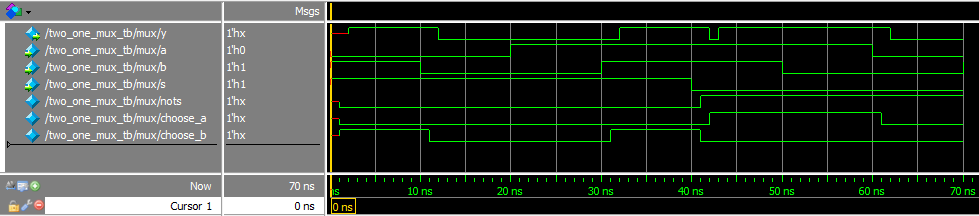
\includegraphics[width=\textwidth]{21mux_wave}
  \caption{2-1 多路选择器}
\end{figure}

可以看到,在 42~ns 时确实出现了静态 1 冒险。

\begin{figure}[H]
  \centering
    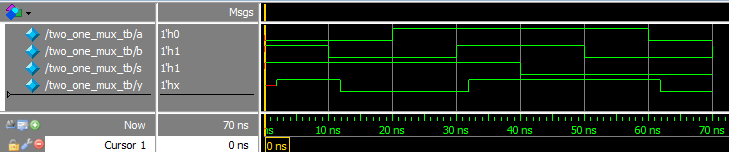
\includegraphics[width=\textwidth]{refined_21mux_wave}
  \caption{消除冒险后的2-1 多路选择器仿真波形}
\end{figure}

从波形中可以看到,在加入了冗余项之后,42~ns 时的静态 1 冒险确实被消除了。(注意这张图中的 y 在最下面,上一张则是在最顶上)

\subsubsection{4-1 多路选择器}
\begin{figure}[H]
  \centering
    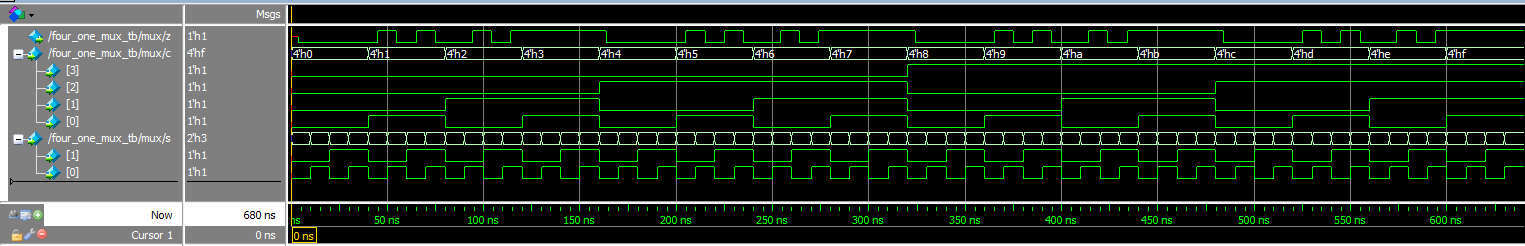
\includegraphics[width=\textwidth]{41mux_wave}
  \caption{4-1 多路选择器仿真波形}
\end{figure}
上面的波形测试了 4-1 多路选择器的所有输入情况,所有有些拥挤…不过结果是对的!


\subsection{三八译码器}
\begin{figure}[H]
  \centering
    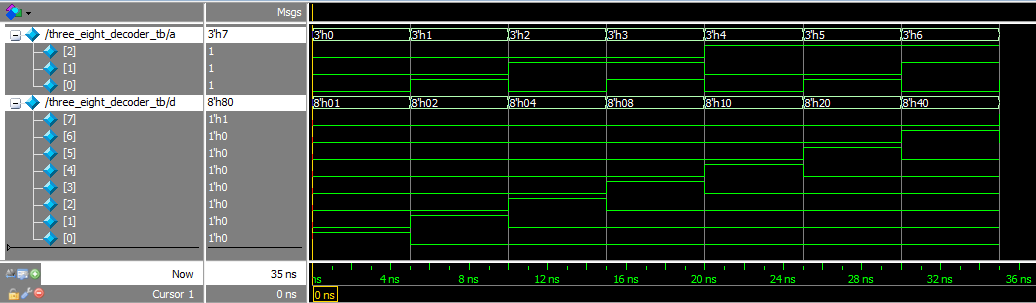
\includegraphics[width=\textwidth]{38decoder_wave}
  \caption{三八译码器仿真波形}
\end{figure}
从下面那个规整的波形可以看出,这确实是个三八译码器= =。


\subsection{移位寄存器}
\begin{figure}[H]
  \centering
    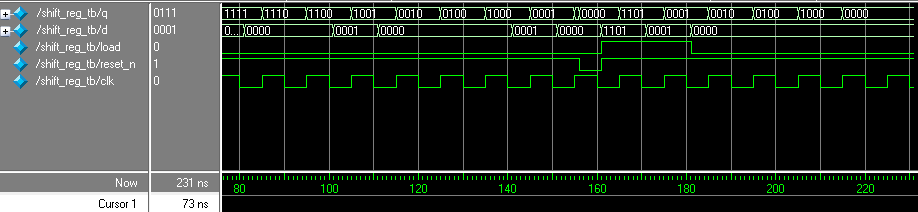
\includegraphics[width=\textwidth]{shift_reg_wave}
  \caption{移位寄存器仿真波形}
\end{figure}

从波形中可以看到,我萌确实实现了寄存器\textasciitilde

要注意,左侧波形是在测试移位功能,中间一段测试了清零功能,最后一段则先后 load 了 1101 和 0001,测试了同步置数的功能。


\end{document}

